\chapter{Data Analysis}
\label{ch:analysis}

\section*{Cosmic Microwave Background cluster lensing}

Cosmic Microwave Background (CMB) photons while passing through intervening galaxy cluster gets lensed and we call this phenomenon as CMB-cluster lensing.
 Lensing remaps the unlensed CMB field based on the angular deflection caused by cluster gravitational potential.
 In mathematical form CMB cluster lensing can be written as the equation below
 \begin{eqnarray}
T(\hat{\textbf{n}})& = & \widetilde{T} (\hat{\textbf{n}} + \vec{\alpha}(\hat{\textbf{n}}))\\
Q(\hat{\textbf{n}}) & = & \widetilde{Q} (\hat{\textbf{n}} + \vec{\alpha}(\hat{\textbf{n}}))\\
U(\hat{\textbf{n}}) & = & \widetilde{U} (\hat{\textbf{n}} + \vec{\alpha}(\hat{\textbf{n}}))
\end{eqnarray}
where $ \widetilde{T}$ is unlensed temperature field, $\widetilde{U}$ and $\widetilde{Q}$ are the unlensed polarisation fields.
$\vec{\alpha}(\hat{\textbf{n}})$ denotes the deflection angle and is directly proportional to the mass of the galaxy cluster.

Lensing signal by an individual cluster is too weak to detect, so we need to stack many clusters to obtain a significant signal.
 For example, the lensing induced distortion due to a $2 \times 10^{14} \ M_{\odot}$ mass galaxy cluster  is $\sim 5.0$ and $0.5 \ \mu K$ in temperature and polarization respectively.
In this chapter, we will discuss various methods available in literature to extract CMB-cluster lensing signal. 
The chapter is organized as follows 

\section{Quadratic Estimator}
%Quadratic Estimator is based on two approximations: gradient approximation and linearization in convergence.

Typical size of galaxy cluster is of the order of few arc minutes. 
Primordial CMB doesn't have power at such small scales due to diffusion damping \cite{Silk} and can be approximated as a gradient. 
Lensing due to galaxy cluster induces a dipole kind of structure oriented along the direction of background gradient with hot and cold spots swapped.
For a given cluster mass and redshift, the magnitude of this dipole scales linearly with the magnitude of the CMB gradient.
This correlation between the unlensed CMB gradient and lensing signal is known as the gradient approximation and is equivalent to
\begin{equation}
T (\hat{n})\approx \tilde{T}+ \nabla T . \vec{\alpha}(\hat{\textbf{n}})
\end{equation}
Below we provide the mathematical formalism for temperature quadratic estimator and it generalises for polarisation.

 Under the gradient approximation, we construct an estimator of lensing convergence by multiplying the lensing map and the gradient map.
The gradient approximation doesn't hold for all fourier modes, only for the modes which are correlated by reconstruction.
Hence we filter maps in the fourier space to isolate modes for which the gradient approximation is valid.
%\begin{equation}
% \hat{k_{l}} = -A_{l} \int d^{2} \hat{n} e^{i\hat{n}.l} Re{\nabla .[G(\hat{n}) L^{*}(\hat{n})]}
 %\end{equation}
 We obtain gradient and lensing maps as follows,
 % $G(\hat{n})$, $L(\hat{n})$ are filtered gradient and lensing maps respectively, $A_{l}$ is the normalisation parameter.
 % We obtain $G(\hat{n})$, $L(\hat{n})$ from the observed temperature map as follows
  \begin{eqnarray}
  L(\hat{n}) = \int \frac{d^{2}l}{(2\pi)^{2}} e^{il .\hat{n}} W^{T}_{l} T_{l}\\
  G(\hat{n}) = \nabla (\int\frac{d^{2}l}{(2\pi)^{2}} e^{il .\hat{n}} W^{TT}_{l} T_{l}   )
  \end{eqnarray}
  where $G(\hat{n})$, $L(\hat{n})$ are filtered gradient and lensing maps and $T_{l}$ is the observed temperature map in fourier space.  
 Fourier filters $W^{T}_{l}$ and $W^{TT}_{l}$ are given by 
 \begin{eqnarray}
 W^{T}_{l} = (C^{TT}_{l} + N^{TT}_{l})^{-1}\\
 W^{TT}_{l} =  \widetilde{C}^{TT}_{l}(C^{TT}_{l} + N^{TT}_{l})^{-1}
 \end{eqnarray}
 where  $\widetilde{C}^{TT}_{l}$,$C^{TT}_{l} $  is the unlensed and large scale structure lensed CMB power spectrum, $ N^{TT}_{l}$ is the noise power spectrum.
 With filtered gradient and lensing maps in hand we can write down the expression for lensing convergence profile as 
 \begin{equation}
 \hat{k_{l}} = -A_{l} \int d^{2} \hat{n} e^{i\hat{n}.l} Re{\nabla .[G(\hat{n}) L^{*}(\hat{n})]}
 \end{equation}
 where $A_{l}$ is the normalisation parameter given by
 \begin{equation}
 \frac{1}{A_{l}} = \frac{2}{l^{2}} \int \frac{d^{2}l_{1}}{4\pi^{2}} (l.l_{1}) W^{TT}_{l} W^{T}_{l} (\tilde{C}^{TT}_{l_{1}}(l.l_{1}) + \tilde{C}^{TT}_{l_{2}}(l.l_{2}))
 \end{equation}
 where $l = l_{1}  + l_{2}$. 
  \subsection{mitigating magnification bias}
Galaxy cluster magnifies the background image and decreases the observed temperature gradient behind it , which leads to a low bias in reconstruction.
The bias is due to the overlap in scales between the unlensed temperature gradient and the lensed temperature field. 
Though wiener filter reduces the bias, it is not removed completely.
We can reduce the bias further by exploiting the prior knowledge on unlensed CMB power spectrum.
 From Fig.~\ref{fig:gradient_cut} which shows the unlensed rms gradient as a function of multipoles, it is evident that most of the power for the gradient map comes from scales below l<2000.
 So by low pass filtering the gradient map, we separate the unlensed temperature gradient and the lensed temperature field with almost no loss in SNR.
 \begin{figure}
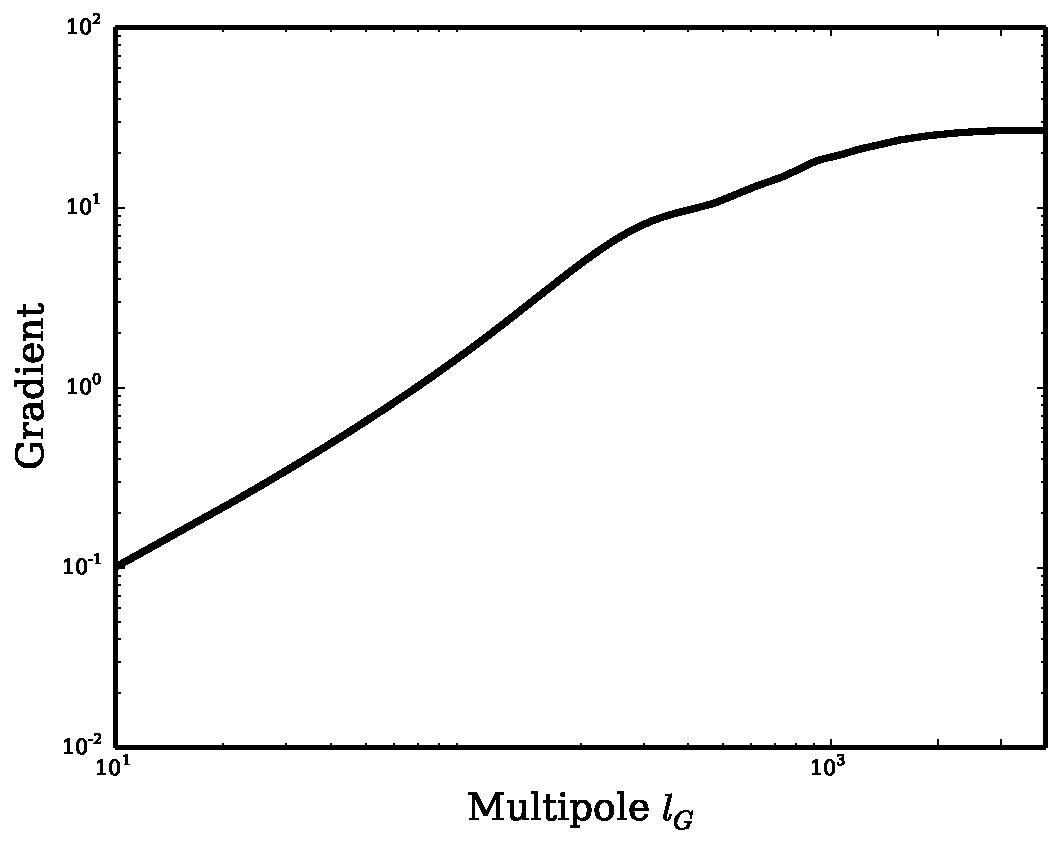
\includegraphics[width=\linewidth]{figs/gradient_cut.pdf}
\caption{Gradient of temperature field as a function of low pass filter l = $l_{G}$. It is dominated by mulitpoles below 2000. \pending{check the magnitude of Grms}}
\label{fig:gradient_cut}
\end{figure}
 \subsection{fitting model}
To obtain the mass of the cluster, we need compare the observed lensing profile to the convergence model generated using an assumed halo mass profile.
 For that we assume the galaxy cluster density to follow Navarro Frenk White (NFW) profile.
 A NFW halo profile is characterized by its scale radius $R_{s}$, the dimensionless concentration parameter c, and the dimensionless charateristic over-density $\delta_{c}$.
 The characteristic over density is defined as the ratio central cluster density to the critical density of the Universe at the cluster redshift.
 In terms of these quantities the NFW halo density profile is written as 
 \begin{equation}
 \rho(r) = \frac{\delta_{c}\rho_{crit,z}}{(\frac{r}{R_{s}})(1 + \frac{r}{R_{s}})^{2}}
 \end{equation} 
 where $\rho_{crit,z}$ is the critical density of the Universe at cluster redshfit.
 
 The lensing convergence profile is the ratio of surface mass density to the critical surface density of the Universe at cluster redshift, $k(x) = \frac{\Sigma(x)}{\Sigma_{crit}}$, where
 \begin{eqnarray}
 \Sigma(x) = 2 \int^{\inf}_{0} \rho(r) ds\\
 \Sigma(crit) = \frac{c^{2}}{4\pi G} \frac{D_{CMB}}{D_{clus} D_{CMB,clus}} 
 \end{eqnarray} 
Here r is the distance from the center, x is the corresponding projection on the plane, is the distance along the line of sight, $D_{CMB}$, $D_{clus}$ are the comoving distances to the CMB and galaxy cluster respectively and $D_{CMB,clus}$ is the distance between the CMB and the cluster.


With model prediction in hand we can write down the likelihood of observing the data as:
\begin{equation}
-2 ln L (k | M) = (k - k_{m})(M) C^{-1} [(k - k_{m})]^{T}
\end{equation}
where k is the observed lensing convergence profile, $k_{m}$ is lensing convergence for NFW profile at mass M, C is the covariance matrix. 

%\section{NFW profile}
The schematic representation of Quadratic Estimator is shown in Fig 2. 
Panel (a) is the 10' X 10' cutout of the observed temperature map, $T_{l}$.
This is filtered in the fourier space \pending{mention equations} to obtain the filtered gradient and lensing maps, shown in panel (b) and (c) respectively.
Lensing convergence profile (panel (c)) is reconstructed by extracting the correlations between lensing and gradient maps.
 \begin{figure}[H]
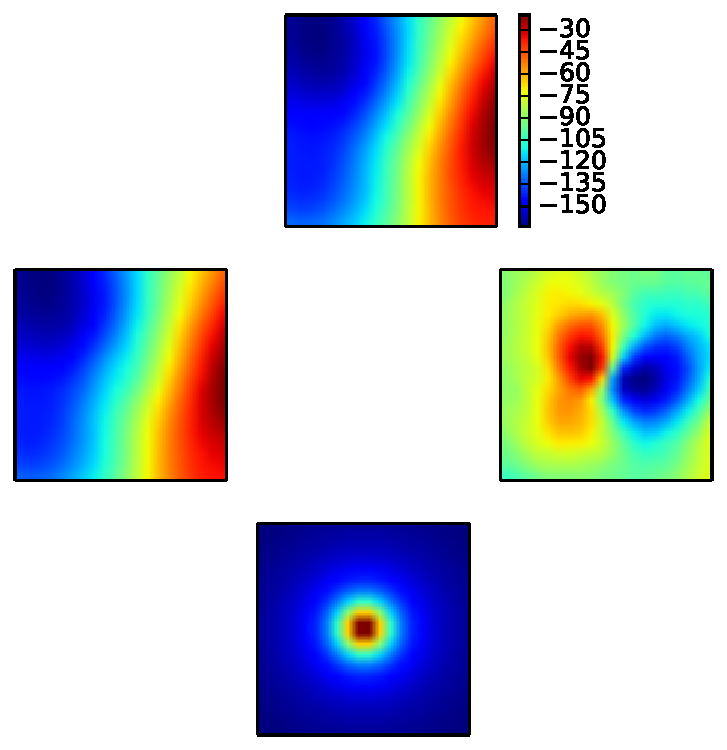
\includegraphics[width=\linewidth]{figs/schematic_rep.pdf}
\caption{Gradient of temperature field as a function of low pass filter l = $l_{G}$. It is dominated by mulitpoles below 2000. \pending{check the magnitude of Grms}}
\label{fig:gradient_cut}
\end{figure}
 
\section{modifications of Quadratic Estimator}
The major foreground in CMB cluster lensing analysis is thermal Sunyaey -Zel'dovich (tSZ) effect. 
tSZ effect is an order of magnitude greater than lensing signal; if not taken into consideration it induces systematic bias and varianace in the final convergence maps.
In this section we describe the modifications of Quadratic Estimator to make it robust to both tSZ induced bias and variance.

\subsection{modified Quadratic Estimator}
While designed to pull the lensing induced correlations, QE is equally sensitive to any other signal present in both G and L maps.
%The major systematic for lensing analysis is thermal Sunyaey -Zel'dovich (tSZ) effect, which is an order of magnitude greater than lensing signal biases the analysis if not taken into account. 
 tSZ present in both maps results in a low bias.
 One way to eliminate tSZ bias is using tSZ free maps, which are constructed by exploiting the frequency dependance of tSZ signal.
 %Previous studies either used a tSZ free map or a more stringent low pass filtering of the gradient map.
 %tSZ is frequency dependent signal and hence we can use multiple frequency channels to eliminate tSZ. 
 However, this results in a increased statistical uncertainty in the reconstructed convergence profile.
 Another way to mitigate the bias is by using a more stringent low pass filter on the gradient map. %; by having a more robust seperation of scales between gradient map and small scale map.
 By having a more robust seperation of scales between gradient map and small scale map.
 While this can reduce the bias significantly, this results in a poor gradient estimation and hence increasing the statistically uncertainty.

 
 During my thesis we came up with a novel approach to completely remove the tSZ bias. 
 Any foreground signal which is present in both the maps will lead to a systematic bias, so by getting rid of the foreground signal in one of the maps (either G or L) should eliminate the bias completely.
  As shown in Fig.~\ref{fig:gradient_cut}, most of the gradient estimation comes from multipoles l <2000 and CMB is not limited by noise at those scales.
  So, natural choice would be to eliminate tSZ in the gradient map by using linear combination of different frequencies. 
  In modified Quadratic Estimator, eqn 3.6 becomes,
  \begin{equation}
   G(\hat{n}) = \nabla (\int\frac{d^{2}l}{(2\pi)^{2}} e^{il .\hat{n}} W^{TT}_{l} T^{SZ_free}_{l}   )
  \end{equation}
  where $T^{SZ_free}_{l} $ is the tSZ-free map.
  \subsection{refinement of modified Quadratic Estimator}
  The sources of variance in the reconstructed convergence maps can be broadly categorised into tSZ variance and non-tSZ variance.
  tSZ variance is due to the tSZ signal present in the small scale map of QE and is independent of the cluster mass.
 On the other hand, tSZ variance increases with mass roughly as $M^{5/3}$.
  
  With modified Quadratic Estimator (mQE) we eliminated the bias due to tSZ, however, tSZ present in the small scale lensing mass induces variance in the reconstructed convergence maps.
 Teh
  \begin{figure}[H]
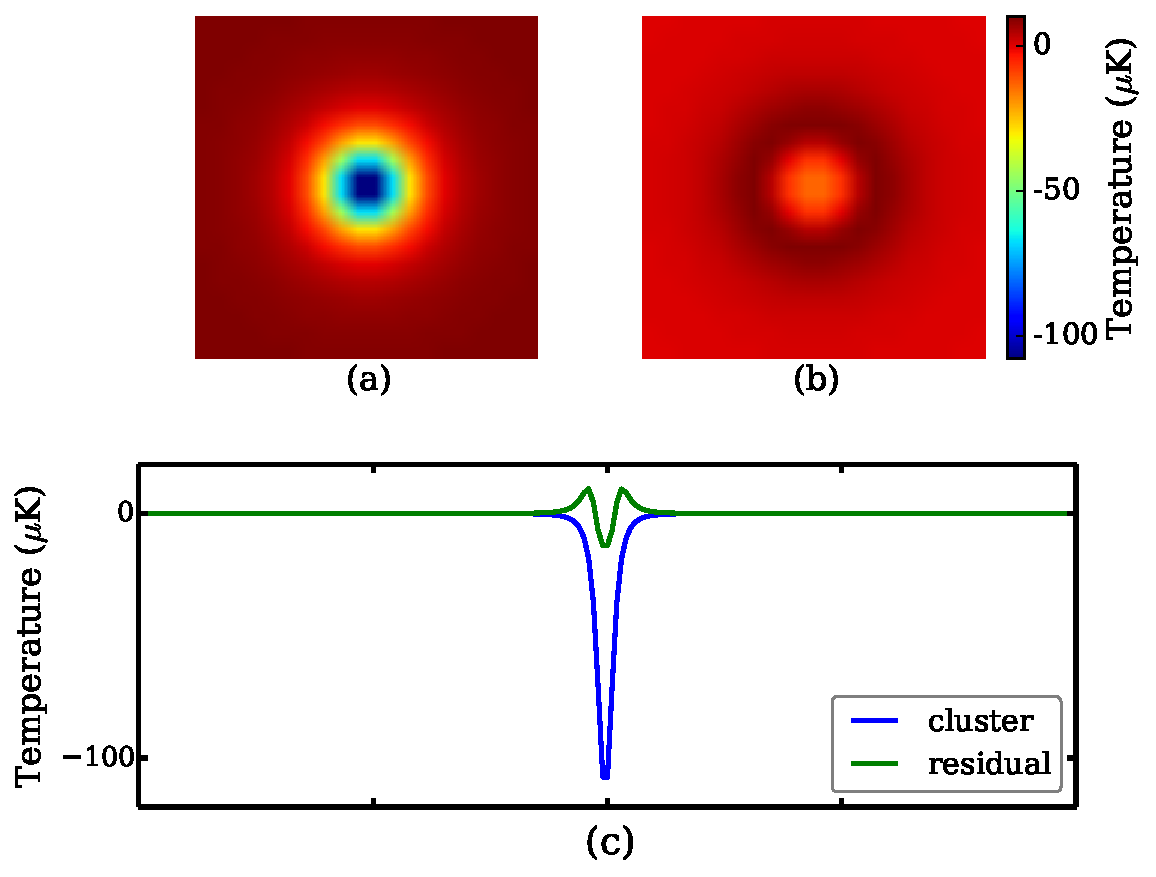
\includegraphics[width=\linewidth]{figs/template_fitting.pdf}
\caption{template}
\label{fig:gradient_cut}
\end{figure}